\section{Вводная лекция}
  \subsection{Операционная система}
  Операционная система -- абстракция, которая связывает различные компоненты компьютера и пользовательские программы.
  
  \subsection{Из каких компонент состоит компьютер?}
  \begin{itemize}
    \item Центральный процессор (CPU или ЦП)
    \item Чипсет и материнская плата
    \item Оперативная память (Random Access Memory = RAM)
    \item Накопители (HDD, SSD, NVMe)
    \item Аудиокарта
    \item Сетевая карта
    \item GPU
    \item Шина (PCI, I2C, ISA)
  \end{itemize}
  
  \subsubsection{Процессор}
  \begin{itemize}
    \item Исполняет команды или \textit{инструкции}
    \item Регистры -- самые быстрые доступные ячейки памяти
    \item Регистры определяют разрядность процессора
    \item Операндами могут быть либо константы, либо регистры, либо ссылки на память
  \end{itemize}
  
  \subsubsection{Оперативная память}
  \begin{itemize}
    \item Random Access Memory
    \item Адресное пространство -- непрерывный массив байт от $0$ до $2^N$, где $N$ -- разрядность процессора ($64$ бита)
    \item В реальности процессоры на текущий момент обычно адресуют не более $48$ бит ($256$ терабайт)
    \item Инструкции процессора расположены также в RAM -- архитектура Фон-Неймана
  \end{itemize}
  
  Сейчас оперативная память работает значительно медленнее процессора (доступ к RAM занимает несколько десятков инструкций процессора). Поэтому внутри процессора есть несколько уровней своей ``оперативной памяти'': L1, L2, L3. Они устроены немного иначе, чем оперативная память, и стоят очень дорого. Если запрашивается доступ к 1 байту, а затем к следующему байту, то второе считывание будет сделано не из оперативной памяти, а из кэша (L1/L2/L3, в зависимости от их наполнения). О том, почему есть несколько уровней кэша, будет рассказано в следующих лекциях.
  Из-за существования кэшей, нам выгодно, чтобы данные лежали ``рядом'' в памяти. Один из примеров: \href{https://levelup.gitconnected.com/c-programming-hacks-4-matrix-multiplication-are-we-doing-it-right-21a9f1cbf53}{ускорение умножения матриц}.
  
  \subsection{Немного ассемблера}
  Ассемблер -- это вид для человека, эти команды -- не процессорные инструкции. На современных процессорах Intel длина инструкции обычно занимает от 1 до 8 байт. В этом курсе будет рассмотрена только архитектура x86. В инструкцию зашивается вся нужная информация: используемые константы, используемые адреса памяти и т.д. Подробнее об этом будет рассказано позже.

\begin{asmminted}
mov rax, qword ptr [rax]
add rax, 2
mov rbx, 1
add rax, rbx
\end{asmminted}

\asmmint{rax}, \asmmint{rbx} -- это регистры процессора. Всего различных регистров общего назначения 16. \newline

Первая инструкция в этом коде берёт адрес регистра \asmmint{rax}, считывает его содержимое, и записывает в него же, в \asmmint{rax}. \newline
Вторая команда прибавляет к содержимому \asmmint{rax} $2$. \newline
Третья команда записывает в \asmmint{rbx} $1$. \newline
Четвертая команда прибавляет \asmmint{rbx} к \asmmint{rax}.
        
    \subsection{Мультизадачность}
    \begin{itemize}
      \item Мультизадачность -- способность системы исполнять несколько задач (процессов) одновременно
      \item Cooperative multitaksing -- процессы добровольно передают управление друг другу
      \item Preemptive multitasking -- процессы вытесянются ОС каждые несколько миллисекунд
    \end{itemize}
    
    Минус cooperative multitasking: если процесс завис, то он не передаст управление дальше, остается только reset.\newline
    Первая Windows, в которой появился multitasking, это Windows 95, до этого был singleprocess MS-DOS.
    
    \subsubsection{Суперскалярность}
    \begin{itemize}
      \item Параллелизм уровня инструкций
      \item Если две инструкции независимы друг от друга, их можно выполнить параллельно
      \item Каждая инструкция состоит из нескольких этапов: fetch, decode, execute, memory access, register write back
      \item CPU pipeline
    \end{itemize}
    Пример процессора без суперскалярности: российский Эльбрус, в котором одна инструкция процессора содержит несколько операций, которые выполняются параллельно. Такой принцип называется VLIW -- Very Long Instruction Word.
    
    \subsubsection{CPU pipeline}
    \begin{figure}[H]
    \centering
  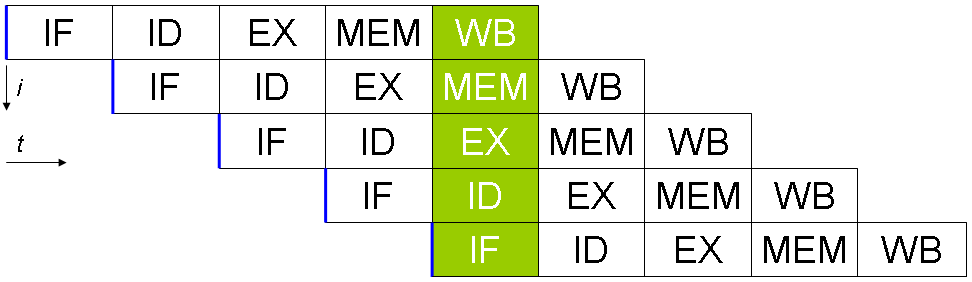
\includegraphics[width=\linewidth]{/Users/user/Downloads/cpu_pipeline.png}
  \caption{CPU pipeline}
  \label{fig:pipeline}
\end{figure}
    
    \subsubsection{Мультипроцессорность}
    \begin{itemize}
      \item Тактовая частота процессоров не растет примерно с 2005 года
      \item Поэтому современные процессоры обычно имеют несколько ядер
      \item \textit{Планировщик (scheduler)} ОС для каждого ядра процессора в каждый момент времени решает какой процесс будет запущен
      \item Возникают проблемы синхронизации
    \end{itemize}
    
    \subsection{Системные вызовы}
    \begin{itemize}
      \item Системные вызовы -- это интерфейс операционной системы для процессов
      \item ABI = application binary interface
      \item SystemV ABI
    \end{itemize}
    Системный вызов -- это очень дорогая операция. У каждой операционной системы свой ABI.
    
    \subsection{POSIX}
    \begin{itemize}
      \item Portable Operating System Interface
      \item Стандарт, описывающий интерфейс операционных систем
      \item Системные вызовы -- часть POSIX, но не все
      \item Например, POSIX описывает как должна быть устроена файловая система
    \end{itemize}
    Иными словами, POSIX -- это стандарт написания операционных систем. Windows -- не POSIX-совместимая система.
    
    \subsection{libc}
    \begin{itemize}
      \item Стандартная библиотека C
      \item Реализует системные вызовы в виде функций C
      \item Ещё куча всяких полезных функций :)
      \item Много реализаций, glibc одна из самых больших
    \end{itemize}
    POSIX определяет, как устроены системные вызовы в виде функций языка C.
    
    \subsubsection{Пример}
\begin{cminted}
int res = read(0, &buf, 1024);
if (res < 0) {
  char* err = strerror(errno);
  // ...
}
\end{cminted}
Функция \cmint{read} возвращает $-1$, если считать не получилось, в противном случае -- количество записанных байт. \newline
\cmint{errno} -- это глобальная переменная (внутри одного потока), в которой хранится последняя ошибка.\newline
Вернуть массив из функции сложно (о причинах будет рассказано в следующих лекциях), поэтому обычно мы просим не вернуть результат, а записать его по некоторому адресу в памяти.

    \subsection{Файловые дескрипторы}
    \begin{itemize}
      \item ``Everything is a file!''
      \item Каждый файл имеет своё имя (или \textit{путь})
      \item Преобразовывать имя файла на каждый сисколл дорого
      \item Сначала нужно получить файловый дескриптор (например, через сисколл \cmint{open})
      \item Все остальные операции без использования пути
    \end{itemize}
    Файловый дескриптор -- это число. Например, $0$ -- это \cmint{stdin}, $1$ -- это \cmint{stdout}, $2$ -- \cmint{stderr}.
